\chapter{Architektur und Aufbau des Prototyps}
\label{cha:arch_pro}
In Kapitel \ref{cha:grdl} wurden die Grundlagen zum MQTT Protokoll und den Sensoren erklärt. Auf Basis dieser Themen wird die Architektur und Aufbau des Prototyps in diesem Kapitel beschrieben. Des weiteren wird erklärt, welche Änderungen in der Architektur vom Prototypen des Praxisprojekts vorgenommen werden.

\section{Architektur des Sofaprototypen}
\label{sec:arch_sofa}
Der Prototyp ist ein im Rahmen des Praxisprojekts entwickeltes System, welches als verteilte Architektur aufgebaut ist. Über drei ESP32 werden Daten von Sensoren erfasst. Die ESPs haben also alle die gleiche Aufgabe.
\newline
Ein Raspberry Pi 2 verarbeitet diese Daten in einem Regelsystem. Mit den verarbeiteten Daten zu festen Regeln werden daraufhin die Endgeräte gesteuert. Dieser Vorgang erfolgt ohne Einfluss der Nutzer. Damit die Sensordaten und die Regeln übertragen werden, wird MQTT verwendet. Mit diesem Prototypen ist es möglich das Personen mit festen Interaktionen die Endgeräte steuern. Damit sind die Interaktionen davon abhängig wie der Nutzer sich auf dem Sofa befindet. Werden die Sensoren in einer anderen Art und Weise verwendet wie es nicht vom Regelsystem vorgesehen ist, so können die erwünschten Ergebnisse nicht erreicht werden.
\newline
Deswegen ändert sich mit der Bachelorarbeit auch das Regelsystem zu einem neuronalen Netz. Außerdem werden die Flex Sensoren nicht mehr für die Liegepositionen eingesetzt. Die Drucksensoren reichen für die Erkennung von der Liegeposition auf den Sitzkissen. 

\begin{figure}[H]
	\centering
		%[natürliche Breite in Pixeln, natürliche Höhe in Pixeln, Abhängigkeit von der Textbreite]
		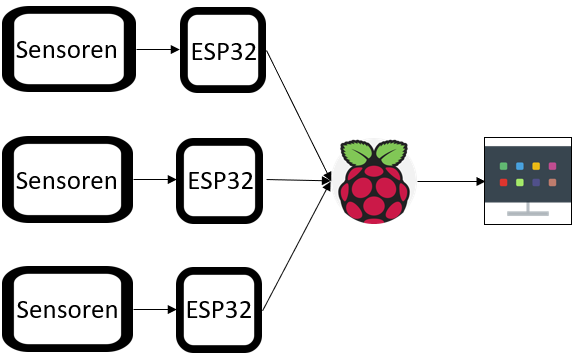
\includegraphics[width=0.6\textwidth]{images/Architektur.png}
	\caption{Abschließende Architektur mit einem Endgerät als Beispiel}
	\label{fig:arch}
\end{figure}

Abbildung \ref{fig:arch} zeigt die Architektur des Prototypen. Als Sensoren werden Ultrasonic Sensoren und Force Sensitive Resistores benutzt. Die Ultrasonic Sensoren messen den Abstand um zu erkennen ob eine Person angelehnt ist. Die FSRs messen anhand des Drucks ob eine Person sitzt, liegt und mit den Armlehnen interagiert. Da dieser Prototyp für ein drei Personen Sofa ausgelegt ist, haben die beiden äußeren ESPs auch jeweils einen FSR für die Armlehnen angeschlossen. Der Raspberry Pi übernimmt zwei Aufgaben und der hier dargestellte Fernseher ist ein Beispiel für ein smartes Endgerät.
\newline
Hinsichtlich dieser Architektur reicht für das System ein lokales Netzwerk. Im Vergleich zu einer Cloud Architekur ist es nicht möglich von außen auf das System zuzugreifen. Da die Steuerung sich auch nur innerhalb des Smart Homes befindet, reicht das lokale Netzwerk auch dafür aus. Eine Cloud Architektur ergibt also nur Sinn, wenn Nutzer außerhalb des Netzwerks im Smart Home auf die Geräte im Smart Home zugreifen wollen.

\section{Regelsystem zur Steuerung der Interaktionen} 
Das neuronale Netz ersetzt das Regelsystem. Dies ist ein statisches System, welches feste Regeln beinhaltet. Die Regeln sind so konzipiert, dass je nach Verwendung der Sensoren eine Regel bzw. ein Code erstellt wird. Der Nachteil dieses Systems ist der feste Aufbau. Wenn eine Regel ausgelöst wird, muss jeder Benutzer immer die gleichen Sensoren auslösen um die Regel zu aktivieren. Das hat den Nachteil für Menschen die das System nicht kennen und zum ersten Mal benutzen. Da sich jede Person anders hinsetzen kann, aber das gleiche Gerät steuern möchte, kann dies nicht vom Regelsystem erkannt werden.
\newline
Mit dem Regelsystem gibt es drei FSR Sensoren und einen Ultrasonic Sensor für die Sitzpositionen im Prototypen. Für die Liegeposition werden zwei Flex Sensoren benutzt. Die Flex Sensoren fallen mit dem einsetzen des neuronalen Netzes weg. Die passiert, weil die Sensoren eine Biegung von mindestens 45 Grad brauchen, damit sie erkennen, dass jemand auf ihnen liegt. Daher werden nun FSRs auch für die Liegepositionen eingebaut. Diese erkennen damit auch zusätzlich ob eine Person sitzt. Somit müssen dann nicht mehr zwei Sensoren in die Sitzkissen eingebaut werden. 

\begin{table}[ht]
	\centering
	\caption[Aufzählung der Regeln des Regelsystems]{Aufzählung der Regeln des Regelsystems}
		\vspace{1.0em}	
	\begin{tabular}{|l|p{7cm}|}
		\hline
		\rowcolor[gray]{0.9}\textbf{Regeln} & \textbf{Beschreibung} \\
		\hline
		\hline
		1 & Alle FSRs und der Ultrasonic Sensor messen Daten \\
		\hline
		2 & Nur der FSR auf dem Sitzkissen misst Daten
		    und der Ultrasonic Sensor \\
		\hline
		3 & Beide FSRs messen Daten \\
		\hline
		4 & Der FSR auf dem Sitzkissen misst Daten \\
		\hline
		5 & Der FSR auf dem Sitzkissen und die beiden Flex Sensoren messen Daten \\
		\hline
		6 & Beide Flex Sensoren messen Sensordaten \\
		\hline
		7 & Ein Flex Sensor und der FSR auf dem Sitzkissen messen Daten \\
		\hline
	\end{tabular}
	\label{tab:tablerules}
\end{table}

\section{Verarbeitung der Daten im ESP und Raspberry Pi}
Kapitel \ref{sec:arch_sofa} zeigt den ESP32 und den Raspberry Pi. Diese sind die Hauptkomponenten zur Verarbeitung der Sensordaten. An einem ESP sind mindestens ein FSR und maximal ein Ultrasonic Sensor angeschlossen. Die Sensordaten werden als Binary Werte vom ESP erfasst und an den MQTT Broker gepublished. Das Python Programm soll diese Daten auf dem RaspberryPi als Subscriber empfangen und verarbeiten. Damit das Python Programm die Sensordaten unterscheiden kann, werden die Sensordaten der jeweiligen Sensoren einzeln gepublished. Das Programm wird als Subscriber vom MQTT Broker erfasst und schickt ihm die Sensorwerte. Um unterscheiden zu können, welcher Wert zu welchem Sensor gehört, hat ein Sensor seinen eigenen Index in einer Liste. Die Daten müssen vor dem Speichern in die Liste noch encoded werden. Über eine Funktion aus der MQTT Bibliothek kann der Binary Wert zu Utf-8 encoded werden. Da das neuronale Netz Integer Werte einliest, muss das encoding stattfinden. Diese Liste speichert mit den Sensorwerten aktuell noch eine unbekannte Position des Nutzers. Daher wird der Listeninhalt bei jeder neuen Position in einer CSV Datei festgehalten und an das neuronale Netz übergeben.
\newline
Sobald das neuronale Netz die Vorhersagen richtig angibt, wird es zusätzlich auf dem Raspberry Pi in das komplette System integriert. Die Verwaltung findet daraufhin über das neuronale Netz statt.

\section{Kommunikation der Sensoren mit dem neuronalen Netz}
Über das MQTT Protokoll findet die Kommunikation statt. Die ESPs schicken über die Publish Funktion die Codes an den MQTT Broker. Der MQTT Broker empfängt die Daten vom Publisher und speichert sie zwischen für die Subscriber. Alle Subscriber empfangen die Daten gleichzeitig und können sie unabhängig voneinander verarbeiten. Als Subscriber dient in diesem Projekt ein Pyton Programm, welches diese Daten für das neuronale Netz empfängt. 
\newline
Die vom neuronalen Netz ausgegebenen Ergebnisse, werden wieder über die Publish Funktion freigegeben. Daraufhin können die Endgeräte diese Ergebnisse verarbeiten und damit gesteuert werden.